\chapter{The Standard Model and Beyond}
\label{chapter:sm}
The Standard Model, the theoretical framework which describes fundamental
particles and their interactions, has a history rooted in the early-to-mid
twentieth century. At its core are two basic groups of particles,
\emph{fermions} and \emph{bosons}, along with three fundamental forces governing
their interactions. Throughout its growth over the last eighty years (as
outlined in~\ref{sec:overview}), the Standard Model has proven to be an
incredibly successful theory, with measurements validating its predictions to a
phenomenal accuracy. Despite its unprecedented level of success, the
Standard Model presents an incomplete description of the universe, as described
in~\ref{sec:shortcomings}, and the search continues for physics that falls
outside of the realm of this theory (\ref{sec:beyond}).

\section{Overview} \label{sec:overview}
The Standard Model unifies the most basic physical interactions into one
overarching framework.  The concept of such a unification can be traced back to
Einstein and beyond, but it is only in the last sixty years that the effort has
really taken shape. 

\subsection{Fundamental Particles} 
\label{sub:funpart}
There are two types of fundamental particles, \emph{fermions} and \emph{bosons}.
Ordinary matter is made up of \emph{fermions}, which carry half-integer spin.
Fermions can be further split into two sub-classes: quarks and leptons.  Quarks
are then classified into three generations of doublets, each generation
consisting of an "up-type" quark with charge $+2/3$ and a ``down-type'' quark
with charge $-1/3$. Quarks are never observed `alone' in nature, due to the laws
of quantum chromodynamics, as explained in~\ref{sub:forces}. Quarks are
susceptible to all three of the fundamental forces included in the Standard
Model -- the strong, weak, and electromagnetic forces. Via the strong force,
quarks form composite color-neutral particles known as \emph{hadrons}, either in
pairs (forming mesons), or in triplets (forming baryons). Protons and neutrons
are the most familiar particle in the hadron family and are composed of two
up-quarks and a down quark or two down-quarks and an up-quark respectively.

Leptons, the other type of fermion, differ in the fact that leptons carry no
color charge. As a result, they do not participate in any strong interactions.
However, the do participate in both electromagnetic (if charged) and weak
interactions. Like quarks, the lepton family is split into three generations,
consisting of the generational type (electron, muon, or tau -- \E, \M, or \T)
plus the doublet partner neutrino. 

\begin{table}[h]
\centering
\begin{tabular}{|c|c|c|c|c|}
\hline
\multicolumn{5}{|c|}{Generation 1} \\
\hline
Particle & Mass (eV/c$^2$) & Charge & T$^{3}$ & Forces\\
\hline
\E          &  5.11$\times$10$^5$   & $\pm 1$        & $+\frac{1}{2}$   & Electromagnetic, weak\\
$\nu_{e}$   &  $<$2.2               & 0              & $-\frac{1}{2}$   & Weak\\
u           &  $2.3\times10^6$      & $+\frac{2}{3}$ & $+\frac{1}{2}$   & Electromagnetic, weak, strong\\
d           &  $4.8\times10^6$      & $-\frac{1}{3}$ & $-\frac{1}{2}$   & Electromagnetic, weak, strong\\
\hline
\hline
\multicolumn{5}{|c|}{Generation 2} \\
\hline
Particle & Mass (eV/c$^2$) & Charge & T$^{3}$ & Forces\\
\hline
\M          & $1.05 \times10^8$     & $\pm 1$           & $+\frac{1}{2}$ & Electromagnetic, weak\\
$\nu_{\mu}$ & $< 1.70\times10^5$    & 0                 & $-\frac{1}{2}$ & Weak\\
c           & $1.3\times10^9$       & $+\frac{2}{3}$    & $+\frac{1}{2}$ & Electromagnetic, weak, strong\\
s           & $9.5\times10^7$       & $-\frac{1}{3}$    & $-\frac{1}{2}$ & Electromagnetic, weak, strong\\
\hline
\hline
\multicolumn{5}{|c|}{Generation 3} \\
\hline
Particle & Mass (eV/c$^2$) & Charge & T$^{3}$ & Forces\\
\hline
\T          & $1.77\times10^9$      & $\pm 1$           & $+\frac{1}{2}$ & Electromagnetic, weak\\
$\nu_{\tau}$& $< 1.55\times10^7$    & 0                 & $-\frac{1}{2}$ & Weak\\
t           & $1.74\times10^{11}$   & $+\frac{2}{3}$    & $+\frac{1}{2}$ & Electromagnetic, weak, strong\\
b           & $4.2\times10^9$       & $-\frac{1}{3}$    & $-\frac{1}{2}$ & Electromagnetic, weak, strong\\
\hline
\end{tabular}
\caption[Fermions and their properties.]{A summary of the generations of fermions and their mass, charge, weak
isospin ($T^{3}$ and the forces which act on them. Nota bene: all right-handed
particles have weak 0 isospin ($T^{3}=0$).}
\label{tab:fermions}
\end{table}

Integer- (or zero-) spin particles known as \emph{bosons} are the particles which
act as force-carriers, as described in~\ref{sub:forces}.  The most common of
these, the photon, is a massless spin-0 particle responsible for governing the
electromagnetic interactions between charged particles.  The \W and \Z bosons
carry the weak force and have charges of $\pm$ 1 and 0 respectively. 
The bosons are summarized in Table~\ref{tab:bosons}.  Gluons, the carriers of
the strong force, are, like photons, electrically neutral and massless. Unlike
the other force-carriers, however, the gluon carries a unit of color and
anti-color, meaning that it is able to self-interact. The implications of this
property are discussed in~\ref{sub:forces}

\begin{table}[h]
\centering
\begin{tabular}{|c|c|c|c|c|}
\hline
\multicolumn{5}{|c|}{Bosons} \\
\hline
Particle & Mass (eV/c$^2$) & Charge & T$^{3}$ & Forces\\
\hline
\Z & $91.2 \times 10^9$ & 0 & 0  & Weak\\
\W & $80.4 \times 10^9$ & $\pm 1$ & $\pm 1$ & Weak\\ 
\photon & 0 & 0 & 0 & Electromagnetic\\ 
g & 0 & 0 & 0 & Strong\\
\hline
\end{tabular}
\caption[Bosons and their properties.]{A list of the force-carrying bosons,
their mass, charge, weak isospin, and the force that they mediate.}
\label{tab:bosons}
\end{table}

\subsection{Fundamental Forces}
\label{sub:forces}
The concept that interactions between fundamental particles can be
attributed to mathematical constructs called fields extends to
Maxwell's formalism of electromagnetism, but it was Feynman, Tomanaga, and
Schwinger who first extended this formalism to the quantum
world. In his theory of quantum electrodynamics (QED,~\cite{Feynman:1950tx}), he
successfully described the electromagnetic interactions between charged
particles as an exchange of massless particles called photons. 

The weak force, carried by \W and \Z bosons, is responsible for those
interactions between fermions that involve charge and flavor changing (such as a
nucleus undergoing $\beta^{-} $ decay through the \Wm-mediated decay
\begin{equation*}
d \rightarrow u + e^{-} + \overline{\nu_{e}}
\end{equation*}

Both the weak and electromagnetic forces have interactions which are governed 
by probability amplitudes of the form:
\begin{equation*}
    \frac{g^4}{\left(q^2c^2-m^2c^4\right)^2}
\end{equation*}
where g is the force's coupling constant, q the momentum transfer of the
interaction, and m the mediating boson's mass. At higher energies (of the order
of $\sim100$~GeV, where the mass of the force-carrying bosons is dwarfed by the
momenta of the particles), the form of the two forces become identical (and
their relative strengths approach equality), suggesting a unification should be
possible between the two.

Sheldon Glashow, Abdus Salam, and Steven Weinberg \cite{Glashow:1961wk} provided
a mathematical basis to this idea, restructuring the forces into an \ewk
algebra.  Within this algebraic structure, the SU(2) operations act only upon
the fermions with left-handed \emph{chirality}, while the U(1) operations act on
those particles which carry hypercharge, Y. This quantum number relates to the
electrical charge, Q, and $T^3$ isospin component through the relation
\begin{equation*}
    Y = 2(Q-T^3)
\end{equation*}
This \ewk algebra describes four physical fields: three vector fields $W_\mu$ which couple to
the weak isospin current (with strength $g$) and one vector field, $B_\mu$ which
couples to the weak hypercharge current with strength proportional to $g'$.
Superposed, these fields describe the physical bosons:
\begin{equation}
\label{eqn:W}
    W_\mu^\pm = \sqrt{\frac{1}{2}}\left(W_\mu^1 \mp i W_\mu^2 \right) \\
\end{equation}
\begin{equation}
\label{eqn:Z}
    Z_\mu = -B_\mu \sin \theta_W + W_\mu^3 \cos \theta_W \\
\end{equation}
\begin{equation}
\label{eqn:g}
    A_\mu = B_\mu \cos \theta_W + W_\mu^3 \sin \theta_W \\
\end{equation}
Where~\ref{eqn:W} describes the weak charged current-carrying \W,~\ref{eqn:Z}
describes the weak neutral current-carrying \Z, and~\ref{eqn:g} describes the
electromagnetic force-carrying photon. $\theta_W$, known as the Weinberg angle,
carries information about the relative coupling strengths in the form
\begin{equation}
    \tan \theta_W = g'/g
\end{equation}.

The third fundamental force, the strong force, describes the interactions
between \emph{quarks} and \emph{gluons}. These are the fundamental particles
(further described in~\ref{sub:funpart}) which make up nuclear matter. The
theory of these interactions, known as quantum chromodynamics, was formulated
in the 1960s.

Because of the gluons' ability to interact with itself, the strong force is
unique in a number of respects. Most notably, the strong force grows stronger as
separation distance between color-charged particles increases. When a quark
sufficiently separates from another, the resulting energy is
enough for other quark-antiquark pairs to pop into existence from the vacuum.
The original quark then combines with these particles. This process, called
hadronization, is driven by \emph{asymptotic freedom} and restricts quarks from
being observed in an unbound state in nature. 

In the algebraic formulation of the Standard Model, the strong force
is represented by a \strong algebra, where C is indicative of the three color
charges (red, green, and blue). In any strong interaction, color must be
conserved, either through adding color and anticolor or one each of the red-
blue- and green- type particles (or anti-red, anti-blue, and anti-green-).

\subsection{Electroweak Symmetry Breaking}
The natural question, giving the unification between the electromagnetic and
weak forces at higher energies is: what causes the two to separate into distinct
forces at lower energies? It is clear that the difference is in the masses of
the force-carrying bosons, but there must be some physical process which gives
rise to the masses of the \W and \Z bosons, breaking the symmetries apparent in
the unified electroweak structure.

The mechanism for this symmetry breaking was proposed independently by
Higgs~\cite{PhysRevLett.13.508}, Englert and Brout~\cite{PhysRevLett.13.321}, and
Guralnik, Hagen, and Kibble~\cite{PhysRevLett.13.585}. The mechanism adds a Higgs
doublet to the electroweak model
\begin{equation*}
    \phi \equiv \left( \begin{array}{c} \phi^+ \\ \phi^0 \end{array} \right)
\end{equation*}
Adding to the potential terms of the form
\begin{equation*}
    V(\phi) = \mu^2\phi^\dagger\phi + \frac{\lambda^2}{2}(\phi^\dagger\phi)^2
\end{equation*}
For $\mu^2<0$, this potential produces a degenerate set of minimal values (see a
quantitative picture in Figure~\ref{fig:higgsPot}) and gives the Higgs field
$\phi$ a non-zero vacuum expectation value. This non-zero vaccuum expectation
value results in mass terms in the Lagrangian corresponding to the \W and \Z
boson.

\begin{figure}[h]
\centering
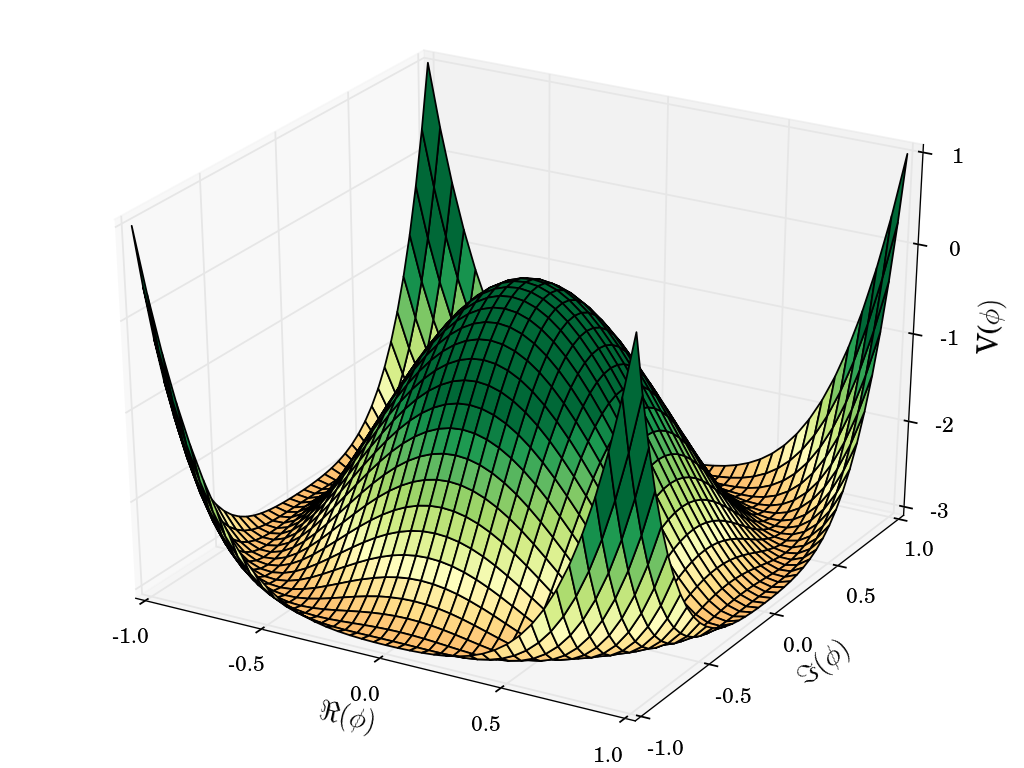
\includegraphics[width=\textwidth]{higgsPot} 
\caption[A quantitative picture of the Higgs potential.]{A quantitative picture
of the Higgs potential, with a ring of degenerate minima.}
\label{fig:higgsPot}
\end{figure}

Although this mechanism neatly explains how mass arises in certain aspects of the
electroweak structure, it is only very recently that a particle resembling the
Higgs boson has been observed (~\cite{CMS:higgsObs},~\cite{ATLAS:higgsObs}), and it has yet to be
conclusively shown whether the observed boson is the Standard Model Higgs or if
it is a Standard Model-like piece of another model. And, as explained
in~\ref{sec:shortcomings} there are certain aspects of the Higgs mechanism that
are left wanting.

\section{Proton-proton collisions}
\label{sec:protonCollisions}
The Large Hadron Collider (LHC) was built with the Higgs boson in mind. The
compositeness of the proton imparts the collisions with in non-trivial physical
ways. The \emph{uud} quark structure of the proton does not accurately describe
the way that the protons interact, as these \emph{valence} quarks are not the
objects that dictate the interactions. As the protons involved in the collisions
get higher and higher in energy, a larger fraction of the protons' momenta is
tied up in the so-called \emph{sea quarks}. These quarks, which can be of any
generation, arise spontaneously as $q\overline q$ pairs pop into existence from
gluons exchanged between the valence quarks. As a result, the LHC has a rich
field of possible initial states; $qq$, $q\overline q$, $qg$, and $gg$ processes
are all possible in the proton-proton collisions. 

Within the Standard Model, the final products in these interactions are governed
by the physical laws of the electroweak and QCD theories. The probability of a
given process occurring is typically expressed in terms of a \emph{cross
section}. The cross section, $\sigma$, is expressed in units of
area\footnote{The standard in particle physics is the \emph{barn}, defined as
$1~b = 10^{-24}~cm^2$} and can be calculated within the Standard Model (or
another relevant quantum field theory). 

These calculations, while often non-trivial, have been conducted for years and
have a well-established methodology. The most general form for a cross section
calculation at the LHC is:

\begin{equation}
    \sigma(pp \rightarrow P + X) = \frac{1}{3} \sum\limits_{q,q'} \int dx_1 dx_2
    f_1(x_1, Q^2) f_2(x_2, Q^2) \sigma_P(\hat s, \hat t, \hat u),
\end{equation}
where $f_1$ and $f_2$ are parton distribution functions and $\sigma_P$ is the
parton-level cross section arising from the matrix element for the process of
interest, P. These matrix elements are themselves calculated based on the rules
of the theory (specifically EWK in this analysis).  The production cross section
of a physical process is heavily dependent upon the forces, particles, and
energies involved. In general, at the energies probed at the LHC, particles
arising via QCD interactions are the most common (due to the high value of
\emph{$\alpha_{s}$}, the size of the strong force coupling.

The cross section provides an easy way to predict the relative rate of physical
processes:
\begin{equation}
    rate = \frac{dN}{dt} = \sigma \cdot \instlum
\end{equation}
Where N is the number of events produced and \instlum is the \emph{instantaneous
luminosity} of the proton beam collisions, explained further
in Section~\ref{section:theLHC}.


\section{Diboson Production} 
Within the Standard Model, a pair of Z bosons can be produced at the LHC either
through quark-antiquark interactions or through gluon interactions (involving a
quark loop)~\ref{fig:zzprod}. Because the standard model prohibits $ZZZ$ (or
$ZZ\gamma$) vertices, %why?
there is no s-channel contribution to the ZZ production
process of the type diagrammed in~\ref{fig:zzatgc}. The quark-antiquark
production mode is the dominant contribution, with the gluon-gluon mode
representing roughly 10\% of the overall cross section~\cite{Campbell:2011jv}.

\begin{figure}[h]
\centering
\unitlength = 1mm
\subfloat{
\begin{fmffile}{qq}
    \begin{fmfgraph*}(60,30)
    \fmfleft{i1,i2}
    \fmfright{o1,o2}
    \fmf{fermion,label=q}{i2,v2}
    \fmf{fermion,label=q}{v2,v1}
    \fmf{fermion,label=$\overline q$}{v1,i1}
    \fmf{photon,label=Z}{v1,o1}
    \fmf{photon,label=Z}{v2,o2}
    \end{fmfgraph*}
    \end{fmffile}
}
\subfloat{
    \begin{fmffile}{gg}
    \begin{fmfgraph*}(60,30)
    \fmfleft{i3,i4}
    \fmfright{o3,o4}
    \fmf{gluon,label=g}{i4,v4}
    \fmf{gluon,label=g}{i3,v3}
    \fmf{fermion,label=q}{v3,v4}
    \fmf{fermion,label=q}{v4,v5}
    \fmf{fermion,label=q}{v5,v6}
    \fmf{fermion,label=q}{v6,v3}
    \fmf{photon,label=Z}{v6,o3}
    \fmf{photon,label=Z}{v5,o4}
    \end{fmfgraph*}
    \end{fmffile}
}
\caption[Standard Model ZZ production]{Production of a ZZ diboson system in the LHC, through qq (left) and gg
production (right)}
\label{fig:zzprod}
\end{figure}

\begin{figure}[h]
\centering
\unitlength = 1mm
\subfloat{
    \begin{fmffile}{atgc}
    \begin{fmfgraph*}(60,30)
        \fmfleft{i6,i5}
    \fmfright{o5,o6}
    \fmf{fermion,label=q}{i5,v7}
    \fmf{fermion,label=$ \overline q$}{v7,i6}
    \fmf{photon,label=$Z,,\gamma$}{v7,v8}
    \fmfblob{0.16w}{v8}
    \fmf{photon,label=Z}{v8,o5}
    \fmf{photon,label=Z}{v8,o6}
    \end{fmfgraph*}
    \end{fmffile}
}
\caption[The SM-forbidden ZZZ (or ZZ$\gamma$ coupling.]{The SM-forbidden neutral triple vertex.}
\label{fig:zzatgc}
\end{figure}


% ------ Higgs production + decays ------
Additionally, a pair of Z bosons may be produced as the decay product of a Higgs
boson. The Higgs boson can be produced in a number of ways, but the dominant
methods are through gluon-gluon fusion and vector boson fusion (colloquially
called the gg and VBF production mechanisms). Additionally, it may be produced
in association with a vector boson (with final state VH) or through $t\overline
t$ fusion. Because the branching ratio of the final states considered in this
thesis are so small, the contributions from these two mechanisms are considered
negligible. Of the two sizable production modes, the $gg$ production
is the dominant mode at the LHC, due to the energies and properties of the
protons involved. The dominant Higgs production mechanisms (with decays to a ZZ
pair) is shown in Figure~\ref{fig:higgsProd}, with cross sections defined in
Table~\ref{tab:higgsProd}. 

\begin{figure}[h] 
\centering 
\unitlength = 1mm
\subfloat{
\subfloat{
    \begin{fmffile}{ggH}
    \begin{fmfgraph*}(60,30)
    \fmfleft{i1,i2}
    \fmfright{o3,o4}
    \fmf{phantom}{i1,v1,d1,o3}
    \fmf{phantom}{i2,v2,d3,o4}
    \fmffreeze
    \fmf{gluon,label=g,l.side=left}{i1,v1}
    \fmf{gluon,label=g,l.side=left}{i2,v2}
    \fmf{fermion,tension=0.5,label=$b,,t$,l.side=left}{v3,v1,v2,v3}
    \fmf{dashes,label=H}{v3,v4}
    \fmf{photon,label=Z}{v4,o3}
    \fmf{photon,label=Z}{v4,o4}
    \end{fmfgraph*}
    \end{fmffile}
}
\begin{fmffile}{vbfH}
    \begin{fmfgraph*}(60,30)
    \fmfleft{i1,i2}
    \fmfright{o1,zo1,zo2,o2}
    \fmf{phantom}{i1,v1,o1}
    \fmf{phantom}{i2,v2,o2}
    \fmffreeze
    \fmf{fermion,label=q,l.side=left}{i1,v1,o1}
    \fmf{fermion,label=q,l.side=left}{i2,v2,o2}
    \fmf{photon,label=$V$,l.side=left}{v1,v3}
    \fmf{photon,label=$V$,l.side=right}{v2,v3}
    \fmf{dashes,label=H}{v3,v4}
    \fmf{photon,label=$Z$,l.side=right}{v4,zo1}
    \fmf{photon,label=$Z$}{v4,zo2}
    \end{fmfgraph*}
    \end{fmffile}
}
\caption[Higgs$\rightarrow$ZZ production.]{The production mechanism of a ZZ system, from a Higgs boson. The $gg$
    (vector boson) fusion is depicted on the left (right).}
\label{fig:higgsProd}
\end{figure}

\begin{table}[h]
\centering
\begin{tabular}{|c|c|c|}
\hline
Production Mode & $\sigma_{8~TeV}$ (pb) & $\sigma_{7~TeV}$ (pb) \\
\hline
$gg \rightarrow H$              & 19.22 & 15.08\\
VBF                             & 1.568 & 1.211\\
WH                              & 0.6782 & 0.5576\\
ZH                              & 0.3843& 0.3077\\
$t\overline t$                  & 0.1271 & 0.0843\\
\hline
\end{tabular}
\caption[Higgs production cross sections at the LHC.]{Higgs boson production cross sections at 7 and 8 TeV for a mass of 126
    GeV.}
\label{tab:higgsProd}
\end{table}

The Higgs boson has well-defined decay characteristics within the Standard Model
(Fig.~\ref{fig:higgsBR}). At the mass of the observed Higgs-like boson
($\sim$126~GeV), the leading decay mode is to a $b\overline b$ pair, accounting
for approximately 56\% of Higgs decays. ZZ decays represent less than 3\% of
total Higgs decays, and only 1\% of those decay into four leptons. However,
given the high resolution with which the electrons and muons can be
reconstructed and the unmatchably clean signature of four leptons, the
$H\rightarrow ZZ \rightarrow \ell \ell \ell' \ell'$ represents a critical
channel in Higgs searches. %2.9% H->ZZ 

\begin{figure}[h]
\centering
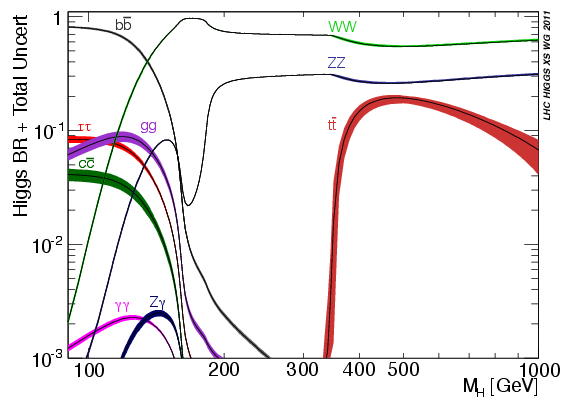
\includegraphics[width=\textwidth]{higgs-BR} %from https://twiki.cern.ch/twiki/bin/view/LHCPhysics/CrossSections
\caption{Higgs decays}
\label{fig:higgsBR}
\end{figure}

The cross sections for each of these ZZ production mechanisms is displayed in
Table~\ref{tab:Zprod}

\begin{table}[h]
\centering
\begin{tabular}{|c|c|c|}
\hline
Production Mode & $\sigma_{8~TeV}$ (pb) & $\sigma_{7~TeV}$ (pb) \\
\hline
$qq \rightarrow ZZ$ + $gg\rightarrow ZZ$ &  7.92   & 6.46 \\
%$gg \rightarrow ZZ$         & & \\
$ H (125~GeV) \rightarrow ZZ$ (total)  & 0.637 & 0.500\\
\hline
\end{tabular}
\caption[ZZ Production cross sections at the LHC.]{ZZ Production cross sections at 7 and 8 TeV. The Higgs production
mechanism includes all contributions (including associated production and
$t\overline t$ fusion).}
\label{tab:Zprod}
\end{table}

\Z bosons are unstable particles and decay into fermion-antifermion pairs. The
majority of these decays are into quarks which immediately decay hadronically.
The next leading Z decay is the decay mode to neutrino pairs, which escape the
detector without interaction. The third, and most relevant within the context of
this thesis, are the decays into lepton pairs. These decays represent roughly
10\% of all Z decays, as demonstrated in Table~\ref{tab:Zdecays}.

\begin{table}[h]
\centering
\begin{tabular}{|c|c|}
\hline
Decay Mode & Fraction (\%) \\
\hline
$e^+e^-$        & $3.363\pm0.004$   \\
$\mu^+\mu^-$    & $3.366\pm0.007$   \\
$\tau^+\tau^-$  & $3.370\pm0.008$   \\
Invisible       & $20.0\pm0.06$     \\
Hadrons         & $69.91\pm0.06$    \\
\hline
\end{tabular}
\caption[Breakdown of decay modes for the \Z boson.]{The branching ratios of the
most common decay modes of the \Z boson. Roughly 10\% of all created \Z bosons
decay leptonically, which is the mode of interest in this thesis.}
\label{tab:Zdecays}
\end{table}

\section{Shortcomings}
\label{sec:shortcomings}
Despite its great successes, the Standard Model is known to be at best an
incomplete theory. Pieces of the theory carry a conspicuously ad-hoc nature, as
the physical constants left floating must be adjusted in a fine balance in order
to cancel divergences in the theory. Similarly, the mechanism of electroweak
symmetry breaking has a non-zero vacuum expectation value only if the $\mu^2$
parameter is negative, which has no physical motivation.

The Standard Model also falls short at being a perfectly unified theory, as it has
little to say about the fourth fundamental force: gravity. Attempts to unify
the Standard Model as it stands today with gravitational forces prove incredibly
difficult, as the scale of the gravitational force is many orders of magnitude
smaller than the others, even at the high energy scales of unification.

Experimental evidence is mounting (~\cite{snoNeutrinoMixing,
superKNeutrinoMixing, dayaNeutrinoMixing}) which indicates
that neutrinos have mass, while the Standard Model in its form presented here
contains massless neutrinos.

The Standard Model, to some extent, seems to provide tension with today's
cosmological theories. It has no components explaining the cosmological phenomena
\emph{dark matter} and \emph{dark energy}. These objects, which compose 23\% and
72\% of the universe's energy content, respectively, have not been accounted for.
There is also no explanation as to why the matter in the universe is composed of 
`ordinary' matter, as opposed to antimatter. The two are suspected to have
existed initially in equal mixing, though only ordinary matter is seen today.

Finally, there's no indication of where the structures and classifications come
from. Why, for example, are there three generations of leptons and quarks
instead of four? Is the current mix of forces `final,' or is it possible to unite
all three forces into one? 

\section{Physics Beyond the Standard Model}
\label{sec:beyond}

Several attempts have been made to answer these some (or all) of these
questions, from the extensions of Supersymmetry, technical to a fully reimagined
grand unified theories, like string theory.  These  theories largely fall
outside of the scope of this thesis, but theories which predict new particles
with ZZ decays (such as those that predict a $Z'$ boson) or neutral triple gauge
couplings have ramifications explained below.
%\subsection{$Z'$ Bosons}
%todo: quick explanation of Z' bosons?

\subsection{Neutral Triple Gauge Couplings}
In the SM, ZZ production proceeds via the $t$- and $u$-channel
$q\overline q$ scattering diagrams, and via gluon-gluon fusion.  The presence of
anomalous neutral trilinear couplings (aTGCs) ZZZ and ZZ$\gamma$
would lead to a sizable enhancement of ZZ final states via $s$-channel
$q\overline q$ scattering as in~\ref{fig:zzatgc}.  A model featuring such
couplings can be constructed by means of an effective
Lagrangian~\cite{Hagiwara:1987tv}.  In this parametrization, two ZZZ couplings
and two ZZ$\gamma$ couplings are allowed by electromagnetic gauge invariance and
Lorentz invariance for on-shell Z bosons.  The form of the vertex function may
be written as: 
\begin{equation}
    \Gamma^{\alpha,\beta,\mu}_{V} = \frac{\hat s-m_V^2}{m_Z^2}\left(
        i f_4^V \left( P^\alpha g^{\mu\beta} \right ) + 
    i f_5^V\epsilon^{\mu\alpha\beta\rho}\left ( q_1-q_2\right)_\rho \right)
\end{equation}.
The couplings are parametrized by two CP-violating (
\ffour ) and two CP-conserving ( \ffive ) complex parameters, all of which are
zero at tree level in the Standard Model (as \ffive~breaks parity conservation).

In general, these couplings do not necessarily conserve partial wave unitarity
at high center-of-mass energies (due to their dependence on$\hat s$). In
previous literature, the $\hat s$ dependence is treated using a form factor,
\begin{equation*} 
    f_i^V(\hat s) = \frac{f_{i0}^V}{\left(1+\frac{\hat s}{\Lambda^2_{NP}}\right)^n}
\end{equation*}
where $\Lambda_{NP}$ is the energy scale at which the new physics manifests
itself and $f_{i0}^V$ is the bare value of the coupling. However, the coupling
values being considered ($\sim0.06$) are unitarity safe through our sensitive
region ($m_{4l} < 1.5~TeV$~\cite{zralek}), and, as a result, no form factor is
assumed. The limits presented in this analysis can thus be interpreted as
restrictions on the `bare' $f_{i0}^V$ couplings.

\subsubsection{Observable manifestations of aTGCs} 
Any indications that these couplings are non-zero are an immediate signal of
physics beyond the standard model. The phenomenological effects are well
described by theorists (for example, \cite{Baur:2000vi}).  The most immediate
effect of anomalous couplings in an increase in the ZZ production cross section,
which would result in a higher-than-anticipated number of observed events.
Additionally, the coupling effects shape the kinematics of the event, becoming
especially pronounced at higher energies. Within the context of this thesis, the
most relevant manifestations are the broad increases in the system's invariant
mass, increases in the \Z transverse momenta, and increased lepton transverse
momenta. The effects on the boson and lepton are exemplified in
figure~\ref{fig:atgcEffects}, reproduced from~\cite{Baur:2000vi}.

Because the effects of the couplings \ffour and \ffive enter the matrix elements
identically, it is impossible to distinguish the two based solely on the effects
explained above. However, it is feasible to comb out some more distinction
between the various couplings given their differing impact on helicity
amplitudes. Specifically, the \ffive couplings produce terms that interfere with
the helicity amplitudes produced by Standard Model couplings. Finally, if
evidence of these couplings were to be found, separation between the leptons
coming from a Z boson (both in the spatial separation and the azimuthal angle
between them) can provide subtle clues to the type (and possibly sign) of the
coupling. The effects can be see in figure~\ref{fig:atgcAngEffects}, reproduced
from~\cite{Baur:2000vi}.

\begin{figure}[h]
\centering
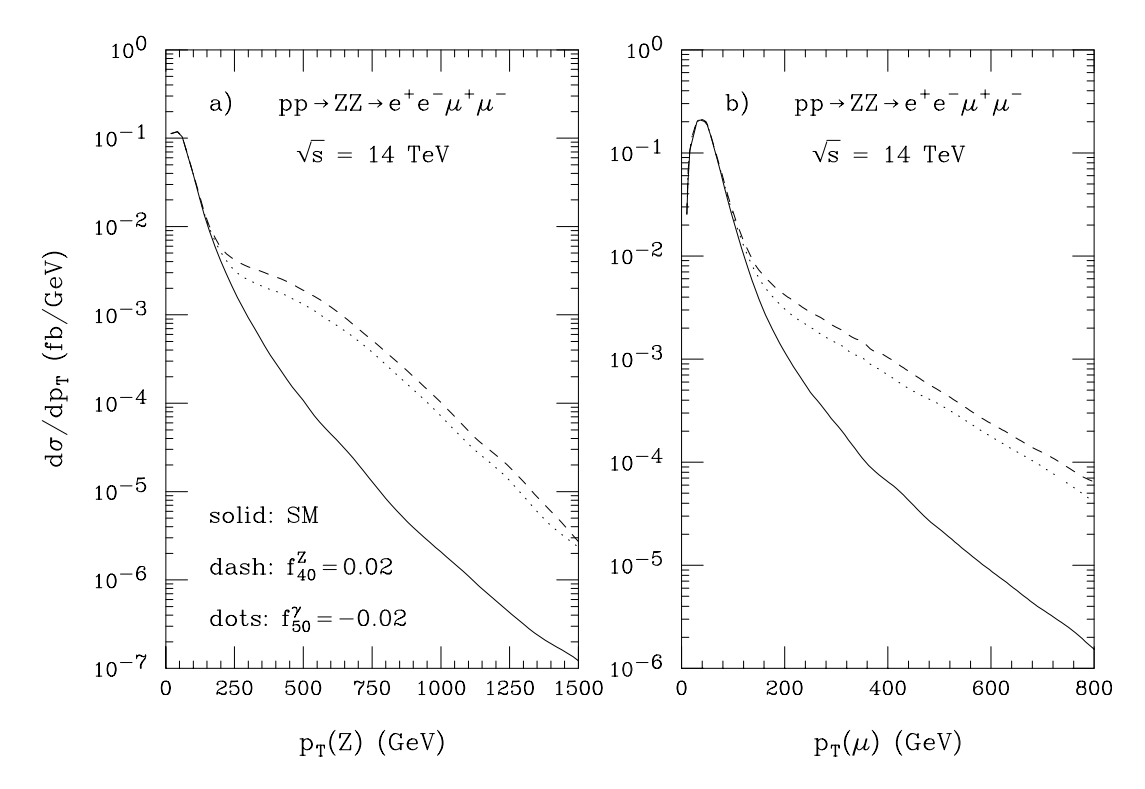
\includegraphics[width=\textwidth]{atgcEffects} 
\caption[Phenomenological effects of aTGCs on boson and lepton
$p_T$.]{Phenomenological effects of aTGCs on boson and lepton $p_T$, reproduced
from~\cite{Baur:2000vi}. Note especially the pronounced high-energy tails
produced by the anomalous couplings.}
\label{fig:atgcEffects}
\end{figure}

\begin{figure}[h]
\centering
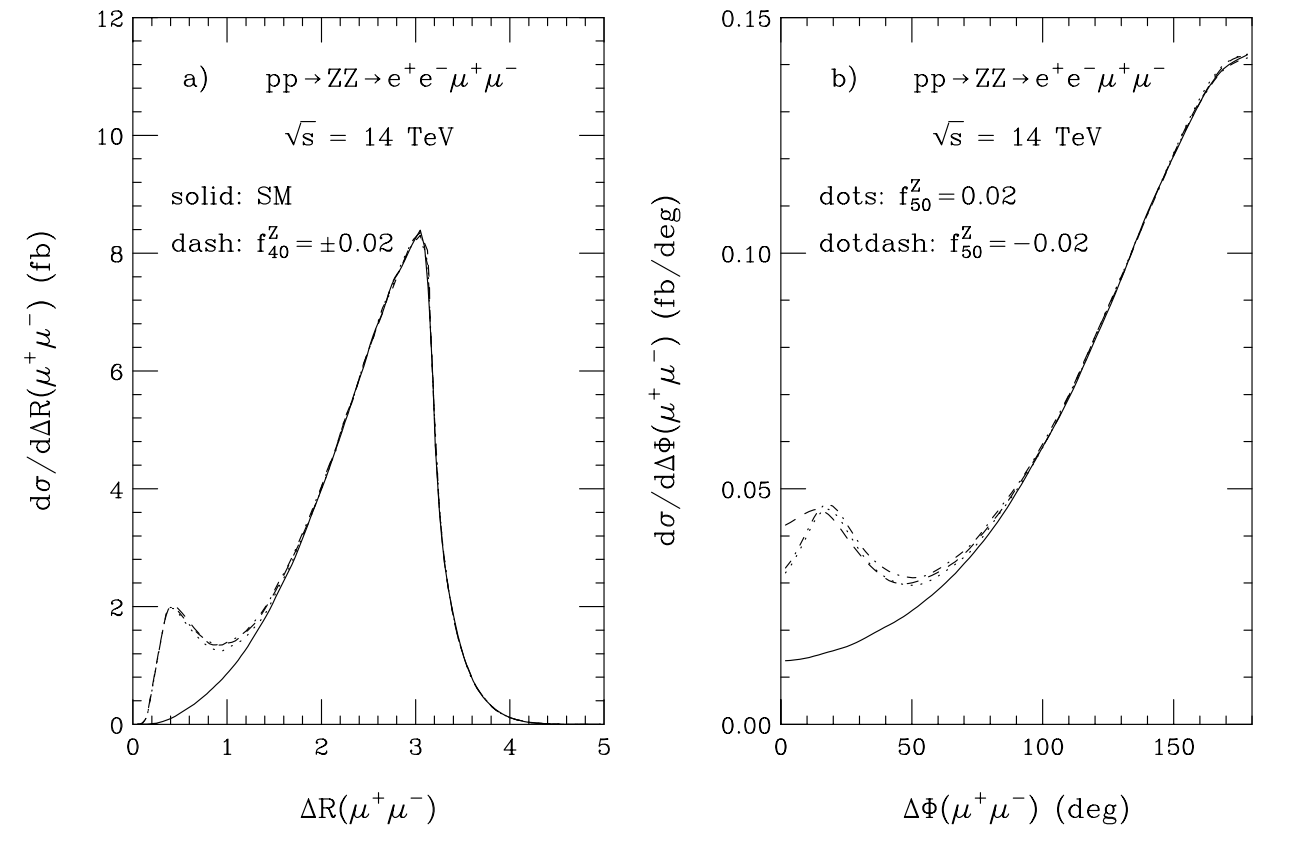
\includegraphics[width=\textwidth]{atgcAngEffects} 
\caption[Phenomenological effects of aTGCs on lepton
separation.]{Phenomenological effects of aTGCs on the separation between leptons, reproduced
from~\cite{Baur:2000vi}. The type, size, and sign of the coupling create slight
differences in the azimuthal angle distribution. Reproduced
from~\cite{Baur:2000vi}.}
\label{fig:atgcAngEffects}
\end{figure}

%todo: what theories predict aTGCs? How would ruling them out change things?
